\chapter{METODOLOGI}
\label{chap:3}

% Ubah bagian-bagian berikut dengan isi dari desain dan implementasi
\begin{figure} [H] 
	\centering
	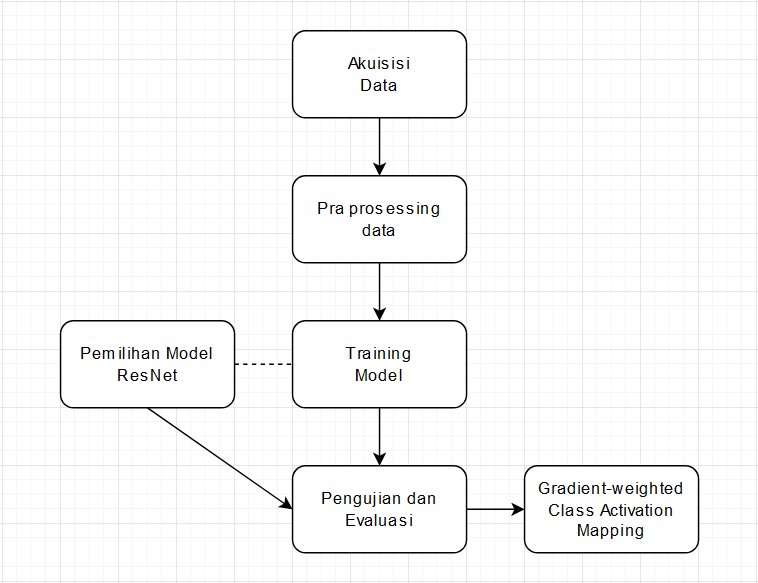
\includegraphics[scale=0.75]{gambar/diagramMethod.png}
	\caption{Diagram blok metodologi}
	\label{fig:diagramMethod}
\end{figure}

\section{Data dan Peralatan}
\label{sec:31}

\subsection{Dataset}
\label{sec:311}
Data yang digunakan dalam penelitian ini adalah data yang diperoleh dari Diabetic Retinopathy Analisis Grand challenge \parencite{drac_challenge_2023_10280359}, berupa citra OCT-\emph{Angiography}.
Untuk persebaran data yang digunakan pada penelitian ini, terdapat pada tabel \ref{table:Datasettraining}

Gambar yang diberikan adalah foto fundus retina yang digunakan untuk evaluasi retinopati diabetik, yang sudah diberi label berupa tingkat keparahan penyakit retinopati diabetik dan sebelumnya sudah melalui proses image assesment sehingga sudah siap digunakan untuk training model.
Foto ini menunjukkan detail dari jaringan pembuluh darah retina, disk optik, dan area makula. Berikut adalah deskripsi rinci dari gambar tersebut:

	\begin{figure}[H]
		\centering
		\subfloat[\centering Non-DR]{{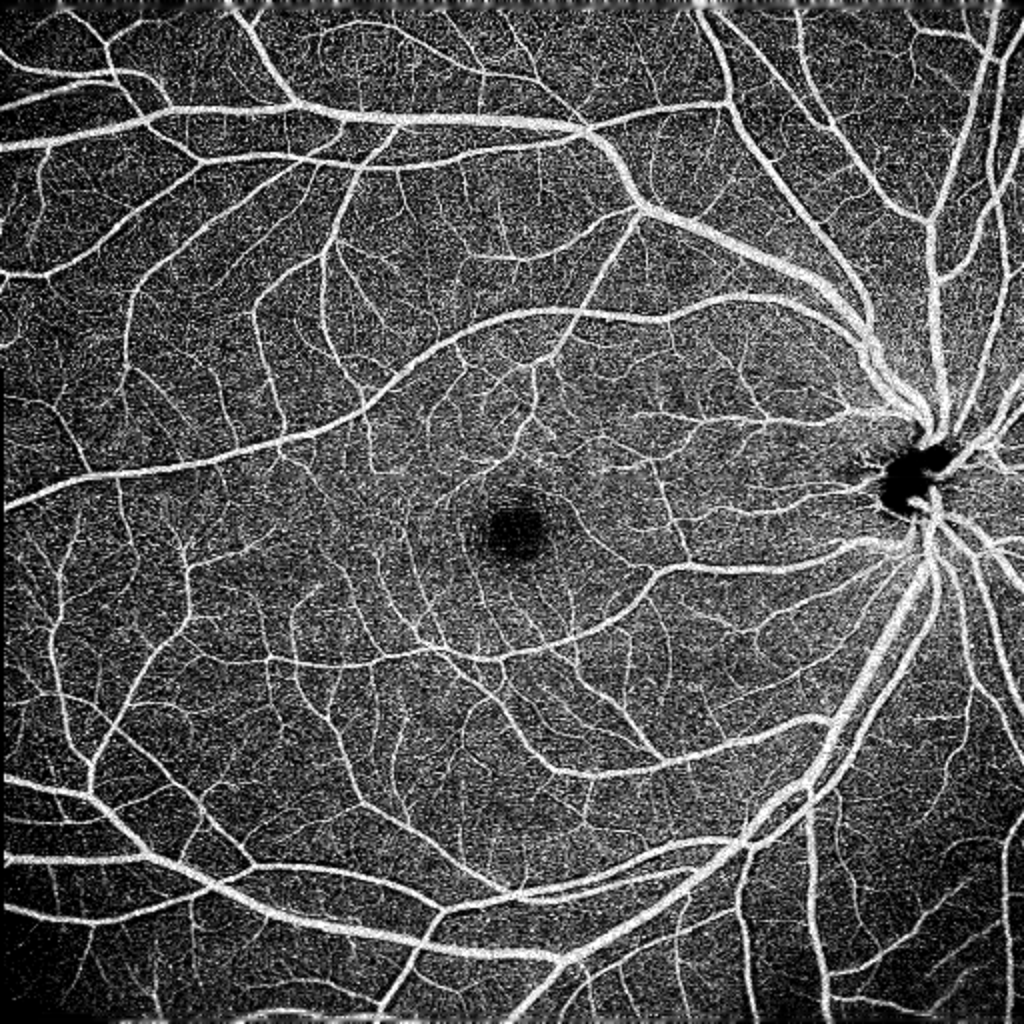
\includegraphics[width=5cm]{gambar/non-DR.png} }}%
		\subfloat[\centering NPDR]{{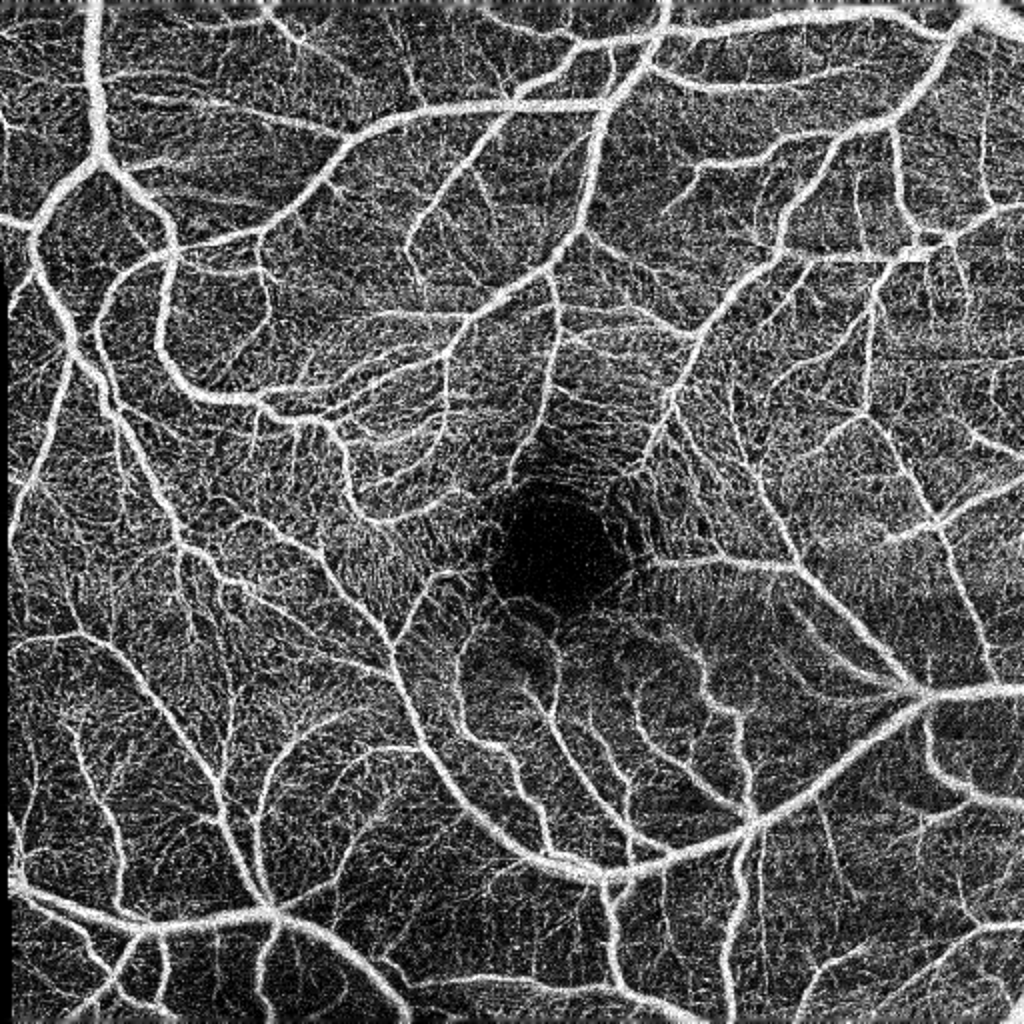
\includegraphics[width=5cm]{gambar/NPDR.png} }}%
		\subfloat[\centering PDR]{{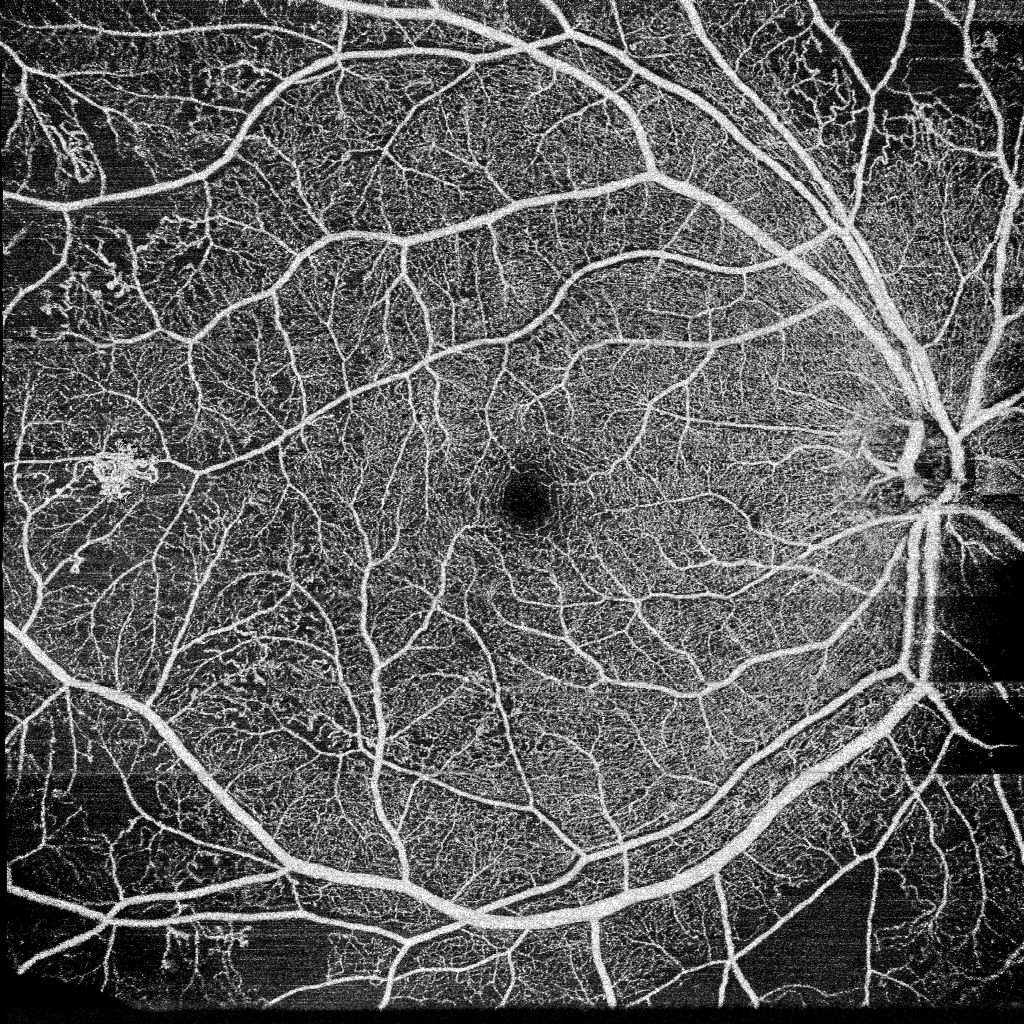
\includegraphics[width=5cm]{gambar/PDR.png} }}%
		\caption{Contoh Data Citra Retina}
		\label{fig:sampleDataset}
	\end{figure}

	\begin{itemize}
		\item \textbf{Struktur Vaskular}: Jaringan pembuluh darah yang jelas terlihat memancar dari disk optik. Pembuluh darah tampak menonjol dan tersebar di seluruh retina.
		\item \textbf{Makula}: Terdapat titik gelap yang terlihat di dekat makula, yang mungkin menunjukkan perubahan retina.
	\end{itemize}
Retinopati diabetik dapat dikategorikan berdasarkan tingkat keparahannya sebagai berikut:

	\begin{enumerate}
		\item Non-DR (0): Non-Diabetic Retinopathy

		\textbf{Karakteristik}: Tidak ada tanda-tanda retinopati diabetik. Retina tampak normal tanpa mikroaneurisma, pendarahan, atau eksudat keras.
		\item NPDR (1): Non-Proliferative Diabetic Retinopathy.

		\textbf{Karakteristik}:
		\begin{itemize}
			\item Kehadiran mikroaneurisma (lesi kecil bulat).\
			\item Pendarahan retina (bercak gelap kecil).
			\item Eksudat keras (bintik-bintik putih terang).
			\item Tidak ada neovaskularisasi.
		\end{itemize}
		\item PDR (2): Proliferative Diabetic Retinopathy

		\textbf{Karakteristik}:
		\begin{itemize}
			\item Kehadiran neovaskularisasi (pertumbuhan pembuluh darah baru yang abnormal).
			\item Mungkin ada pendarahan vitreous (ke dalam humor vitreous mata).
			\item Menunjukkan kondisi yang lebih parah dan berisiko tinggi terhadap kehilangan penglihatan.
		\end{itemize}
	\end{enumerate}

Informasi Dataset dari Tantangan DRAC
Dataset yang digunakan untuk pelatihan dan pengujian terdiri dari:

	\begin{itemize}
		\item Set Pelatihan: 611 gambar
		\item Set Uji: 386 gambar
	\end{itemize}
Gambar-gambar pada set pelatihan, kemudian dipisah kembali menjadi dua set, yaitu set untuk pelatihan dan set untuk validasi dengan jumlah sesuai pada tabel \ref{table:Datasettraining}

\begin{table}[hbtp]
	\begin{center}
	\caption{Tabel distribusi Set untuk Pelatihan dan Validasi}
	\label{table:Datasettraining}
	\begin{tabular}{|l|l|l|l|}
		\hline
		\rowcolor[HTML]{C0C0C0} 
		Label                                                & Klasifikasi & Jumlah & Total                                         \\ \hline
		\rowcolor[HTML]{FFFFFF} 
		\cellcolor[HTML]{FFFFFF}                             & non-DR      & 263    & \cellcolor[HTML]{FFFFFF}                      \\ \cline{2-3}
		\rowcolor[HTML]{FFFFFF} 
		\cellcolor[HTML]{FFFFFF}                             & NPDR        & 169    & \cellcolor[HTML]{FFFFFF}                      \\ \cline{2-3}
		\rowcolor[HTML]{FFFFFF} 
		\multirow{-3}{*}{\cellcolor[HTML]{FFFFFF}Training}   & PDR         & 56     & \multirow{-3}{*}{\cellcolor[HTML]{FFFFFF}488} \\ \hline
		\rowcolor[HTML]{FFFFFF} 
		\cellcolor[HTML]{FFFFFF}                             & non-DR      & 66     & \cellcolor[HTML]{FFFFFF}                      \\ \cline{2-3}
		\rowcolor[HTML]{FFFFFF} 
		\cellcolor[HTML]{FFFFFF}                             & NPDR        & 43     & \cellcolor[HTML]{FFFFFF}                      \\ \cline{2-3}
		\rowcolor[HTML]{FFFFFF} 
		\multirow{-3}{*}{\cellcolor[HTML]{FFFFFF}Validation} & PDR         & 14     & \multirow{-3}{*}{\cellcolor[HTML]{FFFFFF}123} \\ \hline
		\end{tabular}
	\end{center}
\end{table}

Sedangkan gambar pada set uji digunakan untuk mendapatkan penilaian online menggunakan metrik Quadratic Weighted Kappa dengan model dari DRAC sebagai pembandingnya. dan dikarenakan set uji yang diberikan ini tidak memiliki label, maka set ini tidak dapat dipergunakan untuk pengambilan metrik lain seperti \emph{precision, recall}, dan \emph{F1-score}.

\subsection{Peralatan}
\label{sec:312}

Dalam penelitian ini, penulis menggunakan komputer dengan sistem operasi Windows 11 dengan spesifikasi sebagai berikut:

\begin{itemize}
	\item Processor: Intel Core i5 12400F
	\item RAM: 16GB 3200MHz
	\item GPU: NVIDIA GeForce RTX 3060 Ti
	\subitem CUDA Cores: 4864
	\subitem Memory Config: 8 GB GDDR6
\end{itemize}

\subsection{Software}
\label{sec:313}

Software yang digunakan dalam penelitian ini adalah sebagai berikut:
\begin{itemize}
	\item Jupyter Notebook
	\item Visual Studio Code
\end{itemize}

\section{Metode yang Digunakan}
\label{sec:32}

\subsection{Skenario yang digunakan untuk peningkatan performa pelatihan model ResNet}
Dalam penelitian ini, dikarenakan oleh dataset yang sedikit dan terdapat \emph{class} yang kurang representatif, dilakukan metode berikut untuk penyeimbangan dataset.
\begin{itemize}
	\item Default

	Tidak ada Tindakan yang dilakukan untuk menyeimbangkan dataset. Metode ini dilakukan untuk variabel kontrol
	\item Penyesuaian \emph{Class-weight}

	Pada metode ini, dilakukan penambahan weight agar class yang underrepresented memiliki beban lebih tinggi
\end{itemize}

%\subsection{Akuisisi Data}
%\label{sec:321}
%Data yang digunakan dalam penelitian ini adalah data yang diperoleh dari Diabetic Retinopathy Analisis Grand challenge \parencite{drac_challenge_2023_10280359}. Data yang digunakan adalah data citra retina yang sudah diberi label berupa tingkat keparahan penyakit retinopati diabetik yang sebelumnya sudah melalui proses image assesment sehingga sudah siap digunakan untuk training model. Dataset ini berisikan 611 citra OCT-A yang telah diberi label. Dataset ini juga berisikan 386 citra OCT-A yang tidak berlabel untuk dijadikan testing dataset.

\subsection{Pra-pemrosesan Data}
\label{sec:322}
Pra-pemrosesan data dilakukan untuk mempersiapkan data sebelum dilakukan proses pelatihan model. Pra-pemrosesan data yang dilakukan adalah konversi citra retina dari format .jpeg menjadi .png. Hal ini dilakukan karena format .png memiliki ukuran yang lebih kecil dibandingkan dengan format .jpeg. Selain itu, format .png juga tidak mengurangi kualitas citra retina. Pra-pemrosesan data juga dilakukan untuk membagi data menjadi data latih dan data uji. Data latih digunakan untuk melatih model sedangkan data uji digunakan untuk menguji model.

\subsection{Model ResNet}
\label{sec:323}
Model ResNet yang akan digunakan untuk dibandingkan dalam penelitian ini adalah model pre-trained resnet-18, resnet-34, resnet-50, resnet-101, dan resnet-152. Performa model-model tersebut akan disajikan data dari nilai akurasi, \emph{loss}, dan \emph{val\_loss}. 

Dari setiap model yang telah dilatih, akan diambil tiga model, yaitu model dengan nilai akurasi \emph{training} terbaik (\emph{best trained}), nilai akurasi validasi terbaik (\emph{best validated}), serta model epoch terakhir yang dilatih (\emph{last trained}). Tiga model ini kemudian akan dievaluasi tersendiri, dan dibandingkan antara model yang dilatih tanpa menggunakan penyesuaian beban \emph{class}, dan model yang menggunakan penyesuaian beban \emph{class}.

\subsection{Pelatihan Model}
\label{sec:325}
Pelatihan model dilakukan dengan menggunakan metode \emph{transfer learning}. Metode \emph{transfer learning} dilakukan dengan menggunakan model ResNet yang sudah dipilih dan sudah dilatih dengan dataset ImageNet.
Arsitektur model yang digunakan sesuai pada penjelasan bagian \ref{sec:323} dengan menggunakan \emph{hyper-parameter} yang ada pada tabel \ref{tb:hyperParameterTraining}
\begin{table}[hbtp]
	\begin{center}
		\caption{Hyperparameter}
		\label{tb:hyperParameterTraining}
		\begin{tabular}{|
		>{\columncolor[HTML]{C0C0C0}}l |l|lll}
		\cline{1-2}
		Input shape                                         & 224,224,3      &  &  &  \\ \cline{1-2}
		Opimizer                                            & Adam           &  &  &  \\ \cline{1-2}
		Loss Function                                       & Cross Entropy  &  &  &  \\ \cline{1-2}
		Learning Rate                                       & 0.1            &  &  &  \\ \cline{1-2}
		Momentum                                            & 0.9            &  &  &  \\ \cline{1-2}
		\cellcolor[HTML]{C0C0C0}                            & Step size = 10 &  &  &  \\ \cline{2-2}
		\multirow{-2}{*}{\cellcolor[HTML]{C0C0C0}Scheduler} & Gamma = 0.1    &  &  &  \\ \cline{1-2}
		Epoch                                               & 100            &  &  &  \\ \cline{1-2}
		Batch size                                          & 32             &  &  &  \\ \cline{1-2}
		\end{tabular}
	\end{center}
\end{table}

\emph{Input shape} didapatkan dari model pre-training yang dilakukan berdasarkan yang digunakan pada original publishing ResNet \parencite{ResNet}, yaitu 224,224. Jadi, ukuran ini sudah menjadi yang tercanggih. Sehingga ketika dilakukan fine-tuning akan bagus karena konsisten dengan model sebelumnya.

Optimizer ADAM dipilih, karena ADAM dapat dibilang sebagai \emph{optimizer default} dan tidak perlu menghitung optimizer.

Cross Entropy digunakan karena kita melakukan klasifikasi \emph{multiclass} dalam proyek ini. Jadi, cross entropy digunakan untuk menghitung \emph{loss} dari model.

Learning rate \& scheduler

Setelah menghitung \emph{loss}, model akan mengetahui seberapa salahnya. Setelah itu dia akan melakukan backpropagation atau backtracking untuk mengupdate nilai baru setiap node neuron. Tidak ada acuan untuk nilai learning rate dan scheduler. Nilai diambil dari \emph{paper} yang ada, agar tetap konsisten. Dalam penerapannya, nilai ini akan dikalikan dengan turunan \emph{loss} sebagai learning rate. Dan model tersebut ingin mencapai titik terbaik di mana Adam membantu kita mencapai titik terbawah atau terendah dari fungsi tersebut.

Ukuran batch biasanya berhubungan dengan memori. Karena menggabungkan paket kumpulan data menjadi satu, lebih efisien karena satu epoch dapat mempelajari lebih banyak, tetapi membutuhkan lebih banyak memori. Misalnya, ukuran batch 32 berarti begitu memasuki jaringan saraf, akan ada paket data sebanyak 32 gambar.

Momentum dipilih berdasarkan \emph{paper} ResNet \parencite{ResNet}, yang mana dijelaskan betapa mulusnya saat menuruni bukit, yang ada hubungannya dengan optimalisasi \emph{learning rate}.


\subsection{Pengujian dan Evaluasi}
\label{sec:326}
Pengujian dan evaluasi dilakukan dengan menggunakan data uji. Pengujian dan evaluasi dilakukan dengan melihat nilai akurasi, \emph{loss}, dan \emph{val\_loss}. Selain itu, pengujian dan evaluasi juga dilakukan dengan melihat \emph{confusion matrix} dari model yang sudah dilatih, untuk dilihat nilai presisi, recall, dan F1 pada setiap kelasnya, untuk melihat performa model dalam memprediksi tingkat keparahan penyakit retinopati diabetik.

\subsection{Quadratic Weighted Kappa}
Dikarenakan dataset yang digunakan sangatlah kecil, maka metrik QWK juga digunakan untuk menghitung performa dari model. QWK dari model dihitung secara otomatis oleh sistem \emph{online grading} pada website Diabetic Retinopathy Grand Challenge (DRAC) \parencite{drac_challenge_2023_10280359}. Yang mana model yang dihasilkan dari pelatihan pada penelitian ini akan dihitung kesepakatannya dengan model yang ada pada sistem grading DRAC.

Metode grading menggunakan dataset \emph{testing} yang tidak berlabel. Model dari penelitian ini akan memprediksi:
\begin{itemize}
	\item Kelas yang diprediksi
	\item Nilai tensor untuk masing masing kelas (P0, P1, P2)
\end{itemize}
Dari setiap gambar pada dataset \emph{testing}. Hasil prediksi dikeluarkan dalam format .csv, kemudian diunggah ke website dari DRAC.
Setelah itu, sistem akan mengukur hasil QWK dari prediksi yang telah diunggah. Unggahan untuk penilaian terbatas lima kali dalam 24 jam.

\subsection{Gradient-weighted Class Activation Mapping}
\label{sec:327}
Grad-CAM digunakan untuk mengetahui faktor-faktor yang mempengaruhi model dalam memprediksi tingkat keparahan penyakit retinopati diabetik. Grad-CAM bekerja dengan menghitung gradien output model terhadap input, dan kemudian menggunakan gradien tersebut untuk memprediksi area input yang paling berkontribusi pada output model.

%Penelitian ini menggunakan pendekatan sistematis untuk mengkategorikan Non-DR (0), NPDR (1), dan PDR (2) menggunakan Grad-CAM dengan model ResNet-18 default, ResNet-18 class-wegihted, dan ResNet-152 yang telah dilatih sebelumnya. Prosesnya dimulai dengan persiapan model, yang memerlukan adaptasi jaringan saraf ResNet yang sudah ada untuk memenuhi tugas spesifik klasifikasi retinopati diabetik. Model ResNet, yang awalnya dilatih di ImageNet, disesuaikan dengan mengganti lapisan akhir yang terhubung sepenuhnya untuk mengakomodasi tiga kelas yang sesuai dengan berbagai tahap retinopati diabetik. Modifikasi ini memungkinkan jaringan untuk memanfaatkan fitur yang sudah ada sambil berfokus pada kategorisasi gambar retina ke dalam klasifikasi yang diinginkan. Selanjutnya, semua lapisan kecuali lapisan konvolusi terakhir dan lapisan terakhir yang terhubung sepenuhnya dibekukan untuk mempertahankan fitur yang diperoleh, yang merupakan aspek penting untuk klasifikasi yang tepat.
%
%Langkah selanjutnya melibatkan persiapan kumpulan data untuk penilaian. Citra retina menjalani berbagai langkah prapemrosesan seperti konversi ke hitam putih, pengubahan ukuran ke ukuran standar 224x224 pixel, normalisasi, dan konversi ke format tensor. Modifikasi ini memastikan bahwa gambar berada dalam format yang sesuai untuk dimasukkan ke dalam jaringan saraf. Kelas kumpulan data khusus dibuat untuk memfasilitasi pemuatan gambar dari direktori khusus yang mewakili kelas berbeda (Non-DR, NPDR, PDR). Dengan menyusun data dengan cara ini, proses pemuatan data selanjutnya menjadi lebih efektif, memungkinkan pemrosesan batch gambar secara efisien selama evaluasi. Pengaturan ini menjamin bahwa model menerima masukan yang konsisten dan terstandarisasi, yang sangat penting untuk memperoleh hasil klasifikasi yang dapat diandalkan.
%
%Setelah persiapan model dan data, Grad-CAM digunakan untuk membuat interpretasi visual untuk prediksi model. Grad-CAM adalah metode efektif yang mengidentifikasi wilayah tertentu dalam gambar masukan yang berdampak signifikan pada hasil klasifikasi model. Dengan berkonsentrasi pada lapisan konvolusional akhir model ResNet, Grad-CAM menghasilkan heatmap yang mengilustrasikan area gambar retina yang dianggap penting oleh model untuk membedakan antara Non-DR, NPDR, dan PDR. Peta panas ini kemudian ditumpangkan pada gambar asli, sehingga memberikan gambaran visual yang membantu memahami proses pengambilan keputusan model.
%
%Dalam penerapan Grad-CAM, model ResNet yang diadaptasi diinisialisasi dan dialihkan ke mode evaluasi. Grad-CAM secara khusus diarahkan pada lapisan konvolusional akhir model, sebuah langkah penting dalam menghasilkan interpretasi visual yang informatif. Melalui pengaturan ini, gambar masukan diproses untuk menghasilkan heatmap skala abu-abu yang menekankan area signifikan dalam gambar. Peta panas ini dilapiskan ke gambar retina asli untuk menciptakan visualisasi yang menampilkan titik fokus secara efektif. Alat bantu visual tersebut memainkan peran penting dalam memahami dan mengonfirmasi prediksi model, khususnya dalam skenario medis yang memerlukan interpretasi akurat.
%
%Visualisasi ini bertujuan untuk meningkatkan pemahaman prediksi model. Dengan merepresentasikan secara visual elemen gambar retina yang mempengaruhi klasifikasi Non-DR, NPDR, atau PDR, praktisi medis dapat memperoleh wawasan tentang karakteristik mendasar yang membedakan berbagai tahapan retinopati diabetik. Pendekatan metodologis ini tidak hanya meningkatkan transparansi model pembelajaran mendalam namun juga meningkatkan kegunaan praktisnya dalam situasi klinis, di mana alat bantu diagnostik yang dapat diandalkan dan dipahami sangat penting. 
Untuk melakukan klasifikasi Non-DR, NPDR, dan PDR menggunakan Grad-CAM dengan model ResNet-152 yang telah dilatih sebelumnya, dilakukan langkah-langkah berikut:

\subsubsection{Langkah 1: Persiapan Model}
Pertama, model jaringan saraf tiruan dibuat dengan memodifikasi ResNet-152 yang telah dilatih sebelumnya. 
Model ResNet-152 dimuat dengan bobot yang telah dilatih sebelumnya, dan lapisan akhir yang terhubung sepenuhnya disesuaikan untuk menghasilkan tiga kelas, sesuai dengan Non-DR (0), NPDR (1), dan PDR (2). 
Hal ini dilakukan dengan mengatur parameter num\_classes ke 3. 
Semua lapisan kecuali lapisan konvolusi terakhir (layer4) dan lapisan terakhir yang terhubung sepenuhnya dibekukan untuk mempertahankan fitur yang dipelajari dari ImageNet sambil memungkinkan lapisan terakhir beradaptasi dengan tugas klasifikasi retinopati diabetik spesifik. 

\begin{lstlisting}[
	label={lst:gradcam}
  ]
  Buat class DiabeticRetinopathyModel:
  Inisialisasi method class:
	  Muat model ResNet yang telah dilatih sebelumnya
	  Dapatkan jumlah fitur dari lapisan terakhir yang terhubung sepenuhnya
	  Ganti lapisan terakhir yang terhubung sepenuhnya dengan lapisan baru yang memiliki num_classes output
	  Bekukan semua lapisan kecuali lapisan konvolusi terakhir (layer4) dan lapisan terakhir yang terhubung sepenuhnya

  Method forward:
	  Lewatkan input x melalui model ResNet
	  Return output
\end{lstlisting}
%  class DiabeticRetinopathyModel(nn.Module):
%    def __init__(self, num_classes=3):
%        super(DiabeticRetinopathyModel, self).__init__()
%        self.resnet = resnet152(weights=ResNet152_Weights.IMAGENET1K_V2)
%        num_ftrs = self.resnet.fc.in_features
%        self.resnet.fc = nn.Linear(num_ftrs, num_classes)
%        for name, param in self.resnet.named_parameters():
%            if 'layer4' not in name:
%                param.requires_grad = False
%        self.resnet.fc.requires_grad = True
%
%    def forward(self, x):
%        return self.resnet(x)

\subsubsection{Langkah 2: Persiapan Data}
Untuk mempersiapkan dataset untuk evaluasi, gambar diproses dan diubah. 
Hal ini melibatkan pengubahan gambar menjadi skala abu-abu, mengubah ukurannya menjadi 224x224 piksel, menormalkannya, dan mengonversinya menjadi tensor. 
Kelas kumpulan data khusus dibuat untuk memuat gambar dari direktori masing-masing untuk setiap kelas (Non-DR, NPDR, PDR). 
Pemuat data kemudian di-instansiasi untuk memfasilitasi pemrosesan batch gambar selama evaluasi.

\begin{lstlisting}[
	%language=python,
	%caption={}
	label={lst:gradcamstep2}
]
Definisikan transformasi untuk gambar uji:
    Ubah gambar menjadi skala abu-abu dengan 3 output channels
    Ubah ukuran gambar menjadi 224x224 piksel
    Ubah gambar menjadi format tensor
    Normalisasi gambar dengan mean dan standar deviasi 0.5 untuk setiap channel

Kelas DiabeticRetinopathyTestDataset:
    Method __init__(img_dir, transform):
        Tetapkan direktori gambar dan transformasi
        Daftar semua nama file gambar di direktori

    Method __len__:
        Kembalikan jumlah gambar

    Method __getitem__(idx):
        Dapatkan nama file gambar pada indeks
        Muat gambar dari direktori
        Terapkan transformasi pada gambar (jika ada)
        Kembalikan gambar yang telah ditransformasi dan nama filenya

Buat instance dataset untuk setiap kelas:
    Muat gambar dari direktori "dataset/0" dengan transformasi yang telah didefinisikan
    Muat gambar dari direktori "dataset/1" dengan transformasi yang telah didefinisikan
    Muat gambar dari direktori "dataset/2" dengan transformasi yang telah didefinisikan

Buat data loader untuk setiap dataset dengan ukuran batch 1 dan tanpa pengacakan
\end{lstlisting}
%test_transform = transforms.Compose([
%    transforms.Grayscale(num_output_channels=3),
%    transforms.Resize((224, 224)),
%    transforms.ToTensor(),
%    transforms.Normalize(mean=[0.5, 0.5, 0.5], std=[0.5, 0.5, 0.5])
%])
%	class DiabeticRetinopathyTestDataset(Dataset):
%	    def __init__(self, img_dir, transform=None):
%	        self.img_dir = img_dir
%	        self.transform = transform
%	        self.img_list = os.listdir(img_dir)
%
%	    def __len__(self):
%	        return len(self.img_list)
%
%	    def __getitem__(self, idx):
%	        img_filename = self.img_list[idx]
%	        img_path = os.path.join(self.img_dir, img_filename)
%	        image = Image.open(img_path)
%	        if self.transform:
%	            image = self.transform(image)
%	        return image, img_filename
%
%	img_dir_0 = "dataset/0"
%	img_dir_1 = "dataset/1"
%	img_dir_2 = "dataset/2"
%	test_data_0 = DiabeticRetinopathyTestDataset(img_dir_0, test_transform)
%	test_data_1 = DiabeticRetinopathyTestDataset(img_dir_1, test_transform)
%	test_data_2 = DiabeticRetinopathyTestDataset(img_dir_2, test_transform)
%	test_dataloader_0 = DataLoader(test_data_0, batch_size=1, shuffle=False)
%	test_dataloader_1 = DataLoader(test_data_1, batch_size=1, shuffle=False)
%	test_dataloader_2 = DataLoader(test_data_2, batch_size=1, shuffle=False)

\subsubsection{Langkah 3: Menghasilkan Visualisasi Grad-CAM}
Grad-CAM digunakan untuk menghasilkan penjelasan visual untuk prediksi model. Model ResNet-152 yang telah dilatih sebelumnya, yang dimodifikasi untuk klasifikasi retinopati diabetik, dimuat dan diatur ke mode evaluasi. Grad-CAM diterapkan pada lapisan konvolusi terakhir untuk menyoroti daerah dalam gambar input yang penting untuk keputusan klasifikasi. Peta panas yang dihasilkan ditumpangkan pada gambar asli untuk memvisualisasikan area yang diminati.
\begin{lstlisting}[
	%language=python,
	%caption={}
	label={lst:gradcamstep3}
]
Impor library yang diperlukan untuk Grad-CAM dan pemrosesan gambar

Muat model ResNet yang telah dilatih dan dimodifikasi
Atur model ke mode evaluasi
Definisikan lapisan konvolusi terakhir (layer4) sebagai lapisan target untuk Grad-CAM

Inisialisasi Grad-CAM dengan model dan layer target

Tetapkan kelas target untuk visualisasi (misalnya, NPDR)

Hitung heatmap Grad-CAM untuk gambar input
Ekstrak heatmap

Overlay heatmap pada gambar asli untuk membuat visualisasi

\end{lstlisting}
%	from pytorch_grad_cam import GradCAM
%	from pytorch_grad_cam.utils.model_targets import ClassifierOutputTarget
%	from pytorch_grad_cam.utils.image import show_cam_on_image
%	import torch
%
%	model = torch.load("../resnet152val.pth")
%	model.eval()
%	target_layers = [model.resnet.layer4[-1]]
%
%	cam = GradCAM(model=model, target_layers=target_layers)
%
%	targets = [ClassifierOutputTarget(1)]
%	grayscale_cam = cam(input_tensor=image.unsqueeze(0), targets=targets)
%	grayscale_cam = grayscale_cam[0, :]
%	visualization = show_cam_on_image(image_real, grayscale_cam, use_rgb=False)
Dengan mengikuti langkah-langkah metodologi ini, model ini dapat mengklasifikasikan tahapan retinopati diabetik dan memberikan penjelasan visual untuk prediksinya, sehingga membantu dalam penafsiran dan kepercayaan terhadap hasil.